% My own macros
\newcommand{\ensuretext}[1]{\ensuremath{\text{#1}}}
\def\ie{\ensuretext{\textit{i.e.,\xspace}}}
\def\eg{\ensuretext{\textit{e.g.,\xspace}}}

\newcommand{\uder}[2]{\frac{\partial #1}{\partial #2}}
\newcommand{\C}{\ensuremath{\mathbb{C}}}
\newcommand{\CP}{\ensuremath{\mathbb{CP}}}
\newcommand{\GL}[1]{\ensuremath{\mathrm{GL}(#1)}}
\newcommand{\SL}[1]{\ensuremath{\mathrm{SL}(#1)}}
\newcommand{\Q}{\ensuremath{\mathbb{Q}}}
\newcommand{\R}{\ensuremath{\mathbb{R}}}
\newcommand{\RP}{\ensuremath{\mathbb{RP}}}
\newcommand{\Z}{\ensuremath{\mathbb{Z}}}
\newcommand{\med}{\ensuremath{\mathop{\mathrm{med}}}}
\newcommand{\uPr}{\ensuremath{\mathop{\mathrm{Pr}}}}
\newcommand{\uE}{\ensuremath{\mathrm{E}}}
\newcommand{\ucov}[2]{\ensuremath{\mathop{\mathrm{cov}}\left(#1 ,\, #2\right)}}
\newcommand{\ucor}[2]{\ensuremath{\mathop{\mathrm{corr}}\left(#1 ,\, #2\right)}}
\newcommand{\ucorr}[2]{\ensuremath{\mathop{\mathrm{corr}}\left(#1 ,\, #2\right)}}
\newcommand{\uvar}{\ensuremath{\mathop{\mathrm{var}}}}
\newcommand{\ud}{\ensuremath{\mathrm{d}}}
\newcommand{\uProj}{\ensuremath{\mathop{\mathrm{Proj}}}}
\newcommand{\uimply}{\ensuremath{\;\Longrightarrow\;}}
\newcommand{\uequiv}{\ensuremath{\;\Longleftrightarrow\;}}
\newcommand{\uforall}{\textrm{ for all }}
\newcommand{\us}[1]{\ensuremath{\mathrm{Sym}(#1)}}
\newcommand{\uo}[2]{\mathrm{Orb}_{#1}(#2)}
\newcommand{\ustab}[1]{\mathrm{Stab}(#1)}
\newcommand{\uinner}[2]{\ensuremath{\langle #1 ,\; #2 \rangle}}
\newcounter{myN}
\newcommand{\urepeat}[2]{%
  \setcounter{myN}{0}
  \whiledo{\value{myN} < #1}{%
    \stepcounter{myN}#2}}
\newcommand{\uvec}[2][n]{\ensuremath{#2_1, \cdots, #2_{#1}}}
\newcommand{\umark}[1]{\marginpar{%
    \vskip-\baselineskip %raise the marginpar a bit
    \raggedright\footnotesize
    \itshape\hrule\smallskip#1\par\smallskip\hrule}}


%%%%%%%%%%%%%% Front matters

\begin{frame}
  \titlepage
\end{frame}

\begin{frame}
  \frametitle{Outline}
  \tableofcontents
  % You might wish to add the option [pausesections]
\end{frame}

%%%%%%%%%%%%% Main text

\section{Introduction}

\begin{frame} \frametitle{The Roles of Biostatistics in Medical
    Research}
  \begin{itemize}
  \item Point Estimation
    \begin{itemize}
    \item Calculating the mean, variance of a given sample, $\dots$
    \item Making nice tables, plots to visualize a given data.
    \end{itemize}
  \item Hypothesis Testing
    \begin{itemize}
    \item Given a \emph{null hypothesis}, such as ``no difference between the control and treatment group'',
      how likely is our observed differences caused by chance only?
    \item Given some reasonable conditions, such as ``we know there \alert{is} a 1.6 units difference
      between the control and treatment group'', how many observations (patients) do we need
      in order to \alert{reject} the \emph{null hypothesis}? This question is answered by a power calculation.
    \end{itemize}
  \end{itemize}
\end{frame}

\begin{frame} \frametitle{The Roles of Biostatistics in Medical
    Research (Cont.)}
  \begin{itemize}
  \item Modeling
    \begin{itemize}
    \item Linear Regression, causal analysis, making predictions etc.
    \end{itemize}
  \item Other statistical procedures. Quality assurance analysis,
    outlier detection, cluster analysis, dimension reduction, decision
    tree, and many, many more.
  \end{itemize}
\end{frame}

\begin{frame} \frametitle{The Population}
  \begin{itemize}
  \item[Definition] In statistics, a \alert{Population} is the set of all persons, objects or
    events that share some characteristics of interest.
    study.
  \item[Examples] Say you want to study the correlation between blood pressure and smoking.
    \begin{itemize}
    \item all persons that have smoked
    \item all persons with hypertension
    \end{itemize}
  \item[Remark] The population you really care about is \alert{all} (potential)
    smokers in the world, now and in the future. Of course it is not feasible to study
    them one by one, so you decide to study, say 40 of them. These forty constitute a \alert{sample}.
  \end{itemize}
\end{frame}

\begin{frame} \frametitle{The Sample}
  \begin{itemize}
  \item In statistics, a sample is a (usually tiny) fraction of the population that
    is choosen (observed) in a study.
  \item The usefulness of a sample depends on one thing: how well the sample represents
    the population. It in turn depends on two things: the sample size (how many observations) and
    the biasness.
  \item Of course, the larger the sample size the better. But there is always a budget constraint.
    That's why we need a good power calculation.
  \item As for the biasness: randomizing, diversity, common sense. Believe or not, this step is actually
    \alert{not} part of statistics!
  \end{itemize}
\end{frame}

\begin{frame} \frametitle{Types of Data}
  \begin{itemize}
  \item Continuous data, e.g., blood pressure, weight
  \item Discrete data, e.g., number of patients in a hospital
  \item Binary data, a special case of discrete data, e.g., smoker/non-smoker
  \item Nominal data, not numerical, e.g., gender of patients
  \item Ordinal data, a special case of nominal data, with a natural order
  \end{itemize}
\end{frame}

\begin{frame} \frametitle{Types of Data (2)}
  The classification of data by their types are not strict. Example:
  \begin{itemize}
  \item Expensive/Economic: Nominal
  \item Label Expensive as 1, Economic as 0: binary
  \item Very expensive (VE)/expensive (E)/economic (C)/very economic (VC): Nominal again, not binary
  \item VE > E > C > VC, ordinal
  \item Dollar amount: 10, 5, 2, 1 (Unit = \$1000), discrete
  \item Exact dollar amount: 10.321, 5.640, etc, (more or less) continuous
  \end{itemize}
\end{frame}

\section{Descriptive Statistics}

\begin{frame} \frametitle{The Arithmetic Mean}
  This is the most frequently used measure of ``center'' of a sample.
  Def and example: ... \\
  Caution:
  \begin{itemize}
  \item it doesn't apply to nominal data.
  \item sensitive to an ``outlier'' (def/reason of an outlier)
  \item It is very important to know that sample mean is only an
    \alert{approximation} to the population mean we are looking for.
  \end{itemize}
\end{frame}

\begin{frame} \frametitle{The Median}
  \begin{itemize}
  \item Suppose you have a series of n values: $X_1, X_2,  X_n$
  \item The median is defined as
  \item If n is odd: the $(n+1)/2$th largest value
  \item If n is even: the average of the $n/2$th and $(n/2+1)$th largest values
  \item Equal numbers of values on both sides of the median.
  \end{itemize}
\end{frame}

\begin{frame} \frametitle{Comparison of the Mean and the Median}
  \begin{itemize}
  \item Sample: $X_1=3.1, X_2=2.2, X_3=6.7, X_4=1.8$
  \item Mean: $\bar{X} = (X_1+X_2+X_3+X_4)/4=3.45$
  \item Median: the average of 3.1 and 2.2, which is 2.65
  \item Change $X_1$ to $31$ (an outlier)
  \item Mean: 10.425; Median: 4.45
  \item Is it a strength or a weakness? Relation to the normal distribution
  \end{itemize}
\end{frame}

\begin{frame} \frametitle{Et Cetera}
  \begin{itemize}
  \item Modes: most frequently observed point
  \item Geometric Mean: log transformation ==> mean ==> antilogarithm
  \end{itemize}
\end{frame}

\begin{frame} \frametitle{Measure of variation}
  Two samples with the same \alert{center} but different \alert{variation}
  \begin{center}
    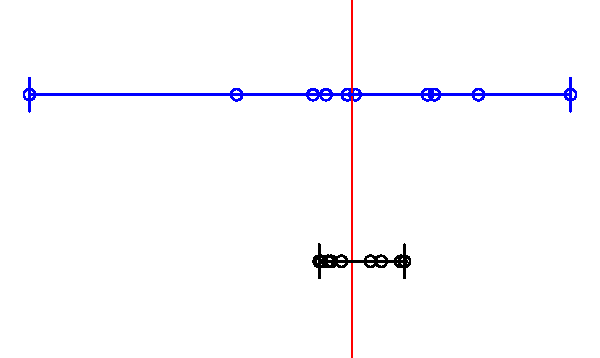
\includegraphics[height=2.4in]{spread.pdf}
  \end{center}
\end{frame}

\begin{frame} \frametitle{The Range}
  \begin{itemize}
  \item Sample: $X_1=3.1, X_2=2.2, X_3=6.7, X_4=1.8$
  \item Minimum: $X_4=1.8$
  \item Maximum: $X_3=6.7$
  \item Range: 6.7-1.8 = 4.9
  \item Sometimes a range is denoted as (1.8, 6.7)
  \item Disadvantage: very sensitive to the extreme values, it also
    depends on the sample size
  \end{itemize}
\end{frame}

\begin{frame} \frametitle{Quantiles}
  \begin{itemize}
  \item Roughly, the $p$th quantile(percentile), denoted as $V_p$, is the value
    such that approximately $p$ percent of the sample observations are less
    than or equal to $V_p$.
  \item See page 18 for a full definition
  \item Median is the 50th quantile.
  \item Quartiles: 25th, 50th, and 75th quantiles.
  \end{itemize}
\end{frame}

\begin{frame} \frametitle{The variance}
  \begin{itemize}
  \item sample variance is defined as
    \begin{equation}
      \label{eq:var}
      \hat{\sigma}^{2} := \frac{ \sum_{i=1}^{n} \left(X_{i} - \bar{X}\right)^{2}}{n-1}.
    \end{equation}
  \item Sample standard deviation: squared root of $\hat{\sigma}^{2}$.
  \end{itemize}
\end{frame}

\begin{frame} \frametitle{Why $n-1$?}
  \begin{itemize}
  \item population variance is $\frac{\sum_{i=1}^{n} (X_i
      -\mu)^{2}}{n}$, when $n$ is really large
  \item By using $\bar{X}$ instead of $\mu$, one \alert{underestimate}
    the variance because $\bar{X}$ is not a perfect estimate of
    $\mu$. We lose one degree of freedom in this step.
  \item The difference between the sample variance and the population
    variance.
  \end{itemize}
\end{frame}

\begin{frame} \frametitle{Graphic Methods}
  \begin{itemize}
  \item Bar Plot/Histogram
  \item Box plots
  \end{itemize}
\end{frame}

\begin{frame} \frametitle{Histogram}
  \begin{center}
    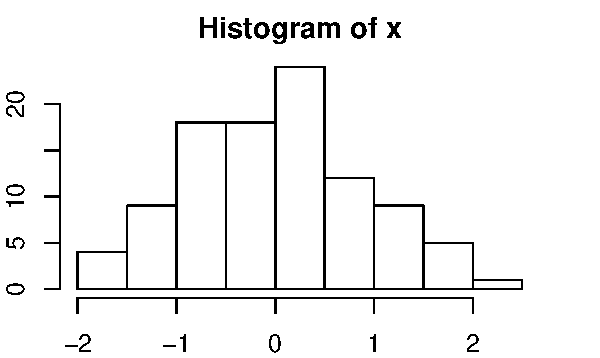
\includegraphics[height=2.4in]{histogram.pdf}
  \end{center}
\end{frame}

\begin{frame} \frametitle{Box Plot}
  The famous \textit{Box and whiskers plot}. min, Q1, median, Q3 and max.
  \begin{center}
    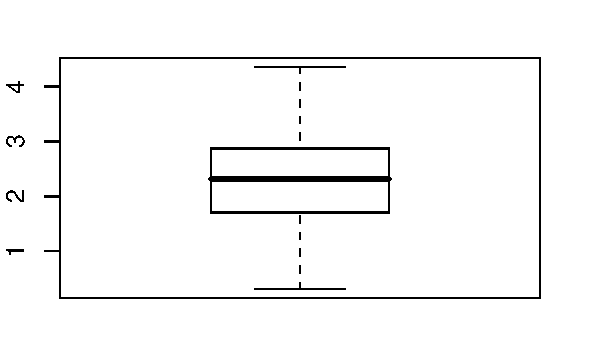
\includegraphics[height=2.0in]{boxplot.pdf}
  \end{center}
\end{frame}

\section{Probability distributions}

\begin{frame}
  \frametitle{Probability distributions}
  \begin{itemize}
  \item Standard Bernoulli distribution (a fair coin). Explain the
    ``coding'' event.
  \item The discrete density function: $f(0)$ and $f(1)$.
  \item General Bernoulli distribution: unfair coin. One parameter:
    success rate.
  \item Binomial distribution and other discrete distributions.
  \end{itemize}
\end{frame}

\begin{frame}
  \frametitle{Continuous distributions}
  \begin{itemize}
  \item Normal distribution. Two parameters: mean and variance (sd).
  \item Non-normal distributions -- thick tail, asymmetry, etc.
  \item Non-normal distributions may have more than two parameters.
    They do not have to be symmetric (mean $\ne$ median).
  \item Large sample approximation (central limit theorem in a
    nutshell).
  \end{itemize}
\end{frame}

\begin{frame}[fragile]
  \frametitle{Normal density and histogram}
  The bell curve (normal distribution) $N(\mu, \sigma^{2})$. Explain
  the relationship between histograms (frequencies) and the idealized
  probability density function (pdf).
  \begin{center}
    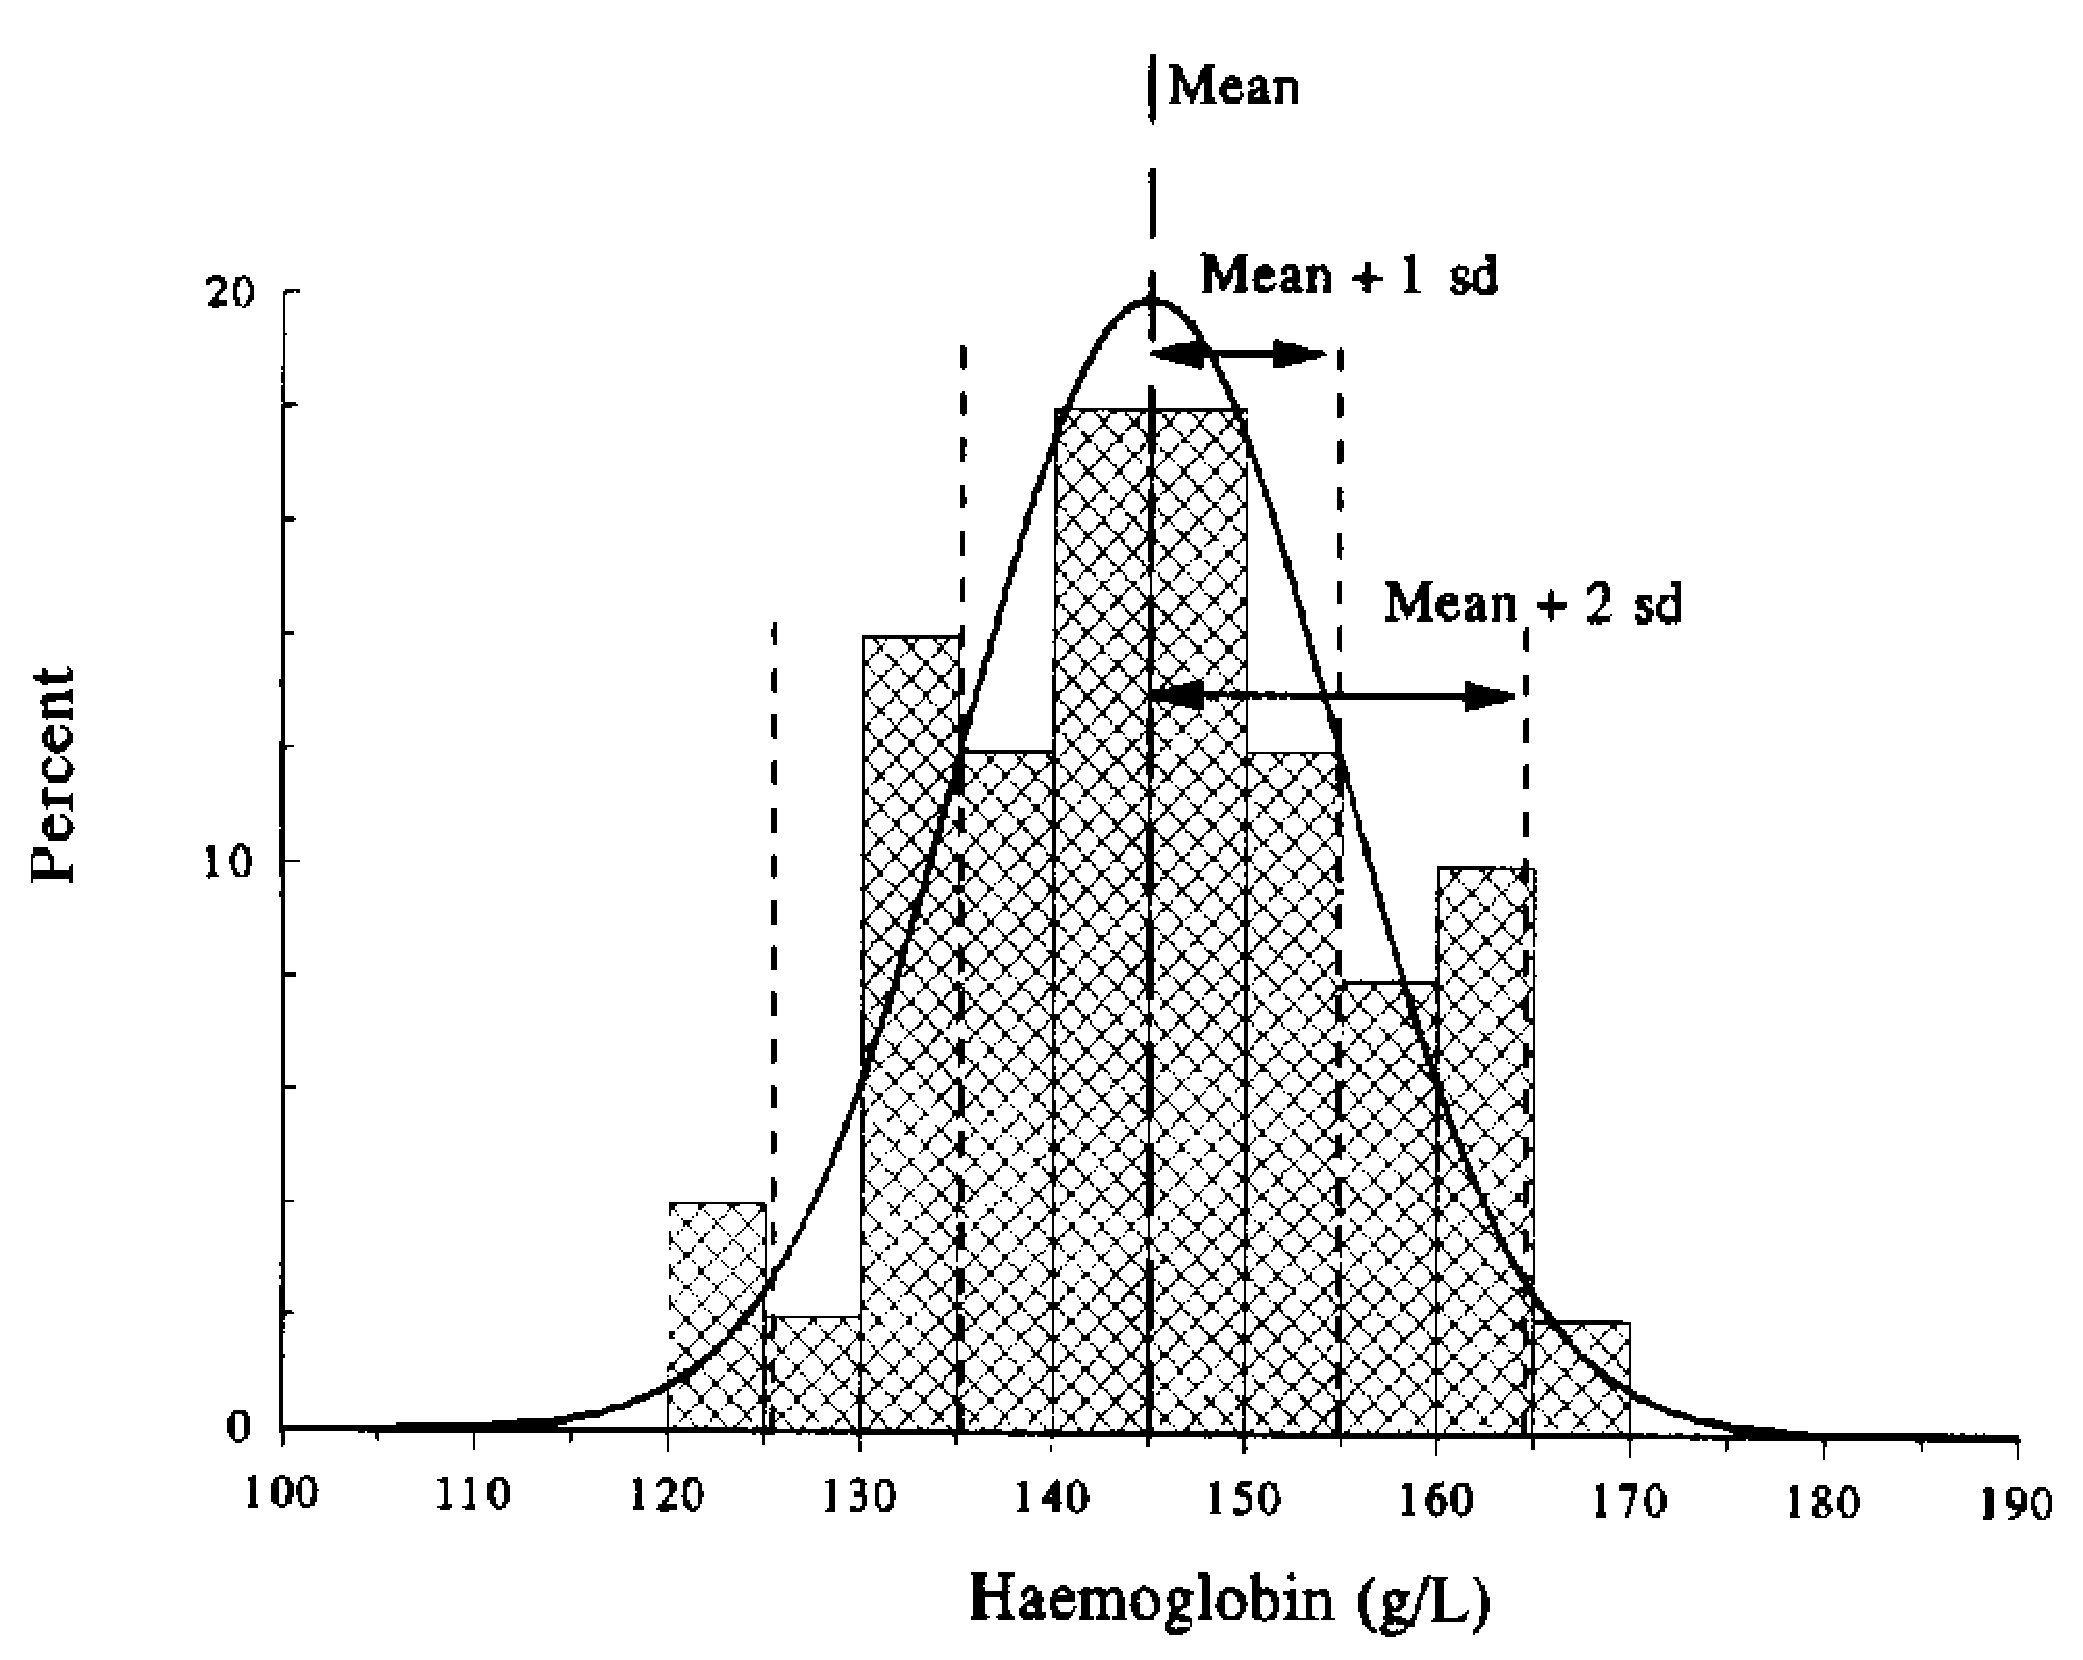
\includegraphics[height=2.0in]{normal}
  \end{center}
\end{frame}

\begin{frame}[fragile]
  \frametitle{Normal density and histogram}
  An example of non-normal distribution ($\Gamma(2,2)$).  Also explain
  the relationship between pdf and cumulative distribution function
  (cdf).
  \begin{center}
    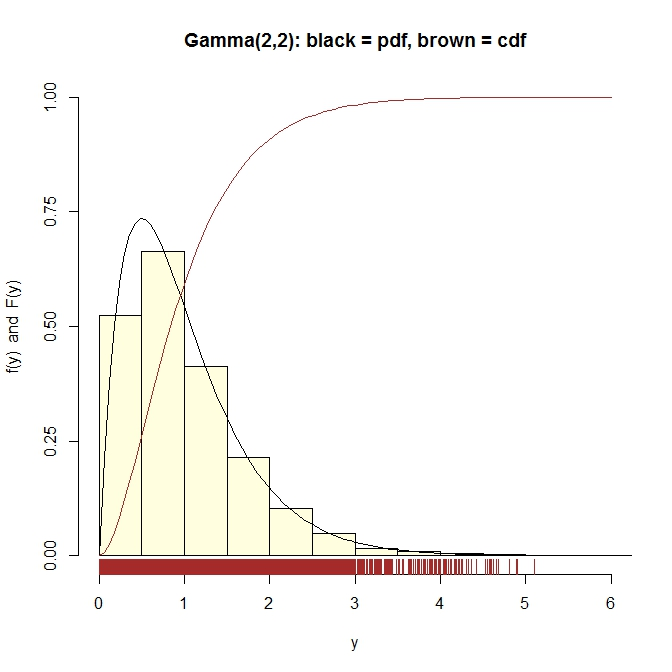
\includegraphics[height=2.0in]{gamma}
  \end{center}
\end{frame}

\section{Point Estimation}

\begin{frame}
  \frametitle{Model-based estimation}
  \begin{itemize}
  \item Definition: an estimator of a parameter $\theta$, usually
    denoted as $\hat{\theta}$, is a quantity defined from the
    \textbf{observations} that \alert{approximates} the unknown value
    of population $\theta$.
  \item $\hat{\theta}$ usually (if not always) differs from the true
    value of $\theta$ (This is a consequence of the sampling
    error).
  \item Heuristically speaking, the smaller this difference is, the
    better this estimator is. How to measure this \alert{difference}
    can get a little complicated, though.
  \end{itemize}
\end{frame}

\begin{frame}
  \frametitle{Examples of estimator}
  \begin{itemize}
  \item The Maximum likelihood estimator (MLE).  Observing the given
    data is ``most likely'' if the true parameter is set to
    $\hat{\theta}^{\mathrm{mle}}$.
  \item Bias-adjusted MLE. $n \to n-1$ in the denominator.
  \item Use moment estimator when MLE is hard to derive/compute.
  \end{itemize}
\end{frame}

\begin{frame}
  \frametitle{Confidence intervals}
  \begin{itemize}
  \item $\hat{\theta}$ is a \alert{random variable} which is an
    approximation of $\theta$. How accurate this approximation is?
    This is why we need confidence intervals for the estimated
    parameters.
  \item Heuristically, a 95\% confidence interval for $\theta$ is an
    interval $I = [C_{1}, C_{2}]$ such that we can say: we are 95\%
    confident that this interval includes the true value of the
    parameter $\theta$.
  \end{itemize}
\end{frame}

\begin{frame}
  \frametitle{Relation to standard error of the mean (SEM)}
  \begin{itemize}
  \item Sometimes, you see a mean estimate reported as $3.12 \pm 0.8$.
  \item This $\pm s$ notation can mean two very different things:
    estimated standard deviation; or the standard error of the mean
    (SEM).
  \item SEM = $\dfrac{\sigma}{\sqrt{n}}$.  Reason:
    $\sigma^{2}(\bar{X}) = \dfrac{\sigma^{2}(X_{i})}{n}$.
  \item The normal approximation: $\bar{X} \pm (2 \cdot \mathrm{SEM})$
    is approximately 95\% CI.
  \end{itemize}
\end{frame}

\section{Hypothesis Testing}

\begin{frame}
  \frametitle{Why we need to test hypotheses}
  \begin{itemize}
  \item Say we want to answer questions like: Is the new treatment
    better than the existing one?
  \item One approach is to estimate the mean response from the new
    treatment group and compare it to that from the old treatment
    group; if the first one is better then we declare the new drug is
    better.
  \item Drawback: Even if there is \alert{no difference}, 1/2 of the
    time we will report new drug better due to \alert{randomness}.
  \end{itemize}
\end{frame}

\begin{frame}
  \frametitle{General concepts}
  \begin{itemize}
  \item The above problem can be expressed in terms of the following
    hypotheses:
    \begin{enumerate}
    \item [$H_{0}$:] The 2 treatments have identical performances.
    \item [$H_{1}$:] The new one has better performances.
    \end{enumerate}
    Here $H_{0}$ is the null hypothesis and $H_{1}$ is the alternative
    hypothesis.
  \item Note that in practice, most of time we test the following
    \alert{two-sided} alternative hypothesis instead.
  \item [$H_{1}$:] The 2 treatments have different performances.
  \end{itemize}
\end{frame}

\begin{frame}
  \frametitle{Decisions}
  \begin{itemize}
  \item A test may have 2 possible outcomes
    \begin{enumerate}
    \item We accept $H_{0}$ (The 2 treatments have identical
      performances).
    \item We reject $H_{1}$ and accept $H_{1}$ (The 2 treatments have
      different performances).
    \end{enumerate}
  \end{itemize}
\end{frame}

\begin{frame}
  \frametitle{Type I, II error, testing power}
  \begin{tabular}{|l|c|c|}
    & Accept $H_0$ & Reject $H_0$ \\
    \hline
    $H_0$  & True Negative & False Positive, type I error) \\
    \hline
    $H_1$  & False Negative, type II error & True Positive) \\
  \end{tabular}
\end{frame}

\begin{frame}
  \frametitle{Type I error and statistical power}
  \begin{itemize}
  \item The probability of making a type I error is often denoted as
    $\alpha$.
  \item It's commonly referred to as the \alert{significant level} of the test.
  \item The probability of making a type II error is often denoted as
    $\beta$.
  \item The \alert{statistical power} of the test is defined as
    $1-\beta$, which is the probability of rejecting $H_{0}$ if
    $H_{1}$ is true.
  \end{itemize}
\end{frame}

\begin{frame}
  \frametitle{Two group comparison with unknown variance}
  \begin{itemize}
  \item A natural way to test $H_{0}$ versus $H_{1}$ is to use mean
    differences, $D = \bar{X}^{A} - bar{X}^{B}$.
  \item Is $D = -12.88$ significant or not?
  \item Answer: We need to know the \emph{variance}.  For example,
    12.88 pounds of mean body weight difference may be significant;
    12.88 \emph{grams} of difference may be trivial.
  \item A lot of hypothesis tests rely on some sort of
    ``signal-to-noise ratio'' statistic to make inference.
  \end{itemize}
\end{frame}

\begin{frame}
  \frametitle{Two sample student $t$-statistic}
  \begin{itemize}
  \item Definition
    \begin{equation}
      \label{eq:t}
      t = \frac{\bar{\mathbf{x}}^{(A)}-\bar{\mathbf{x}}^{(B)}} {\sqrt{s^2(\frac{1}{n_{A}}+\frac{1}{n_{B}})}}.
    \end{equation}
    where $s^{2}$ is the estimated variance using data pooled from both
    groups.
  \item Under normal assumption, $t \sim T(n_{A}+n_{B}-2)$, a Student's
    $t$-distribution with $n_{A}+n_{B}-2$ degrees of freedom, which is
    very similar to a standard normal distribution when sample size is
    large. (Why?)
  \end{itemize}
\end{frame}

\begin{frame}
  \frametitle{Inference}
  We can check the theoretical distribution of $T(n_{A}+n_{B}-2)$ and
  reject $H_{0}$ if the value of $t$ is very ``unlikely''.
  \begin{center}
    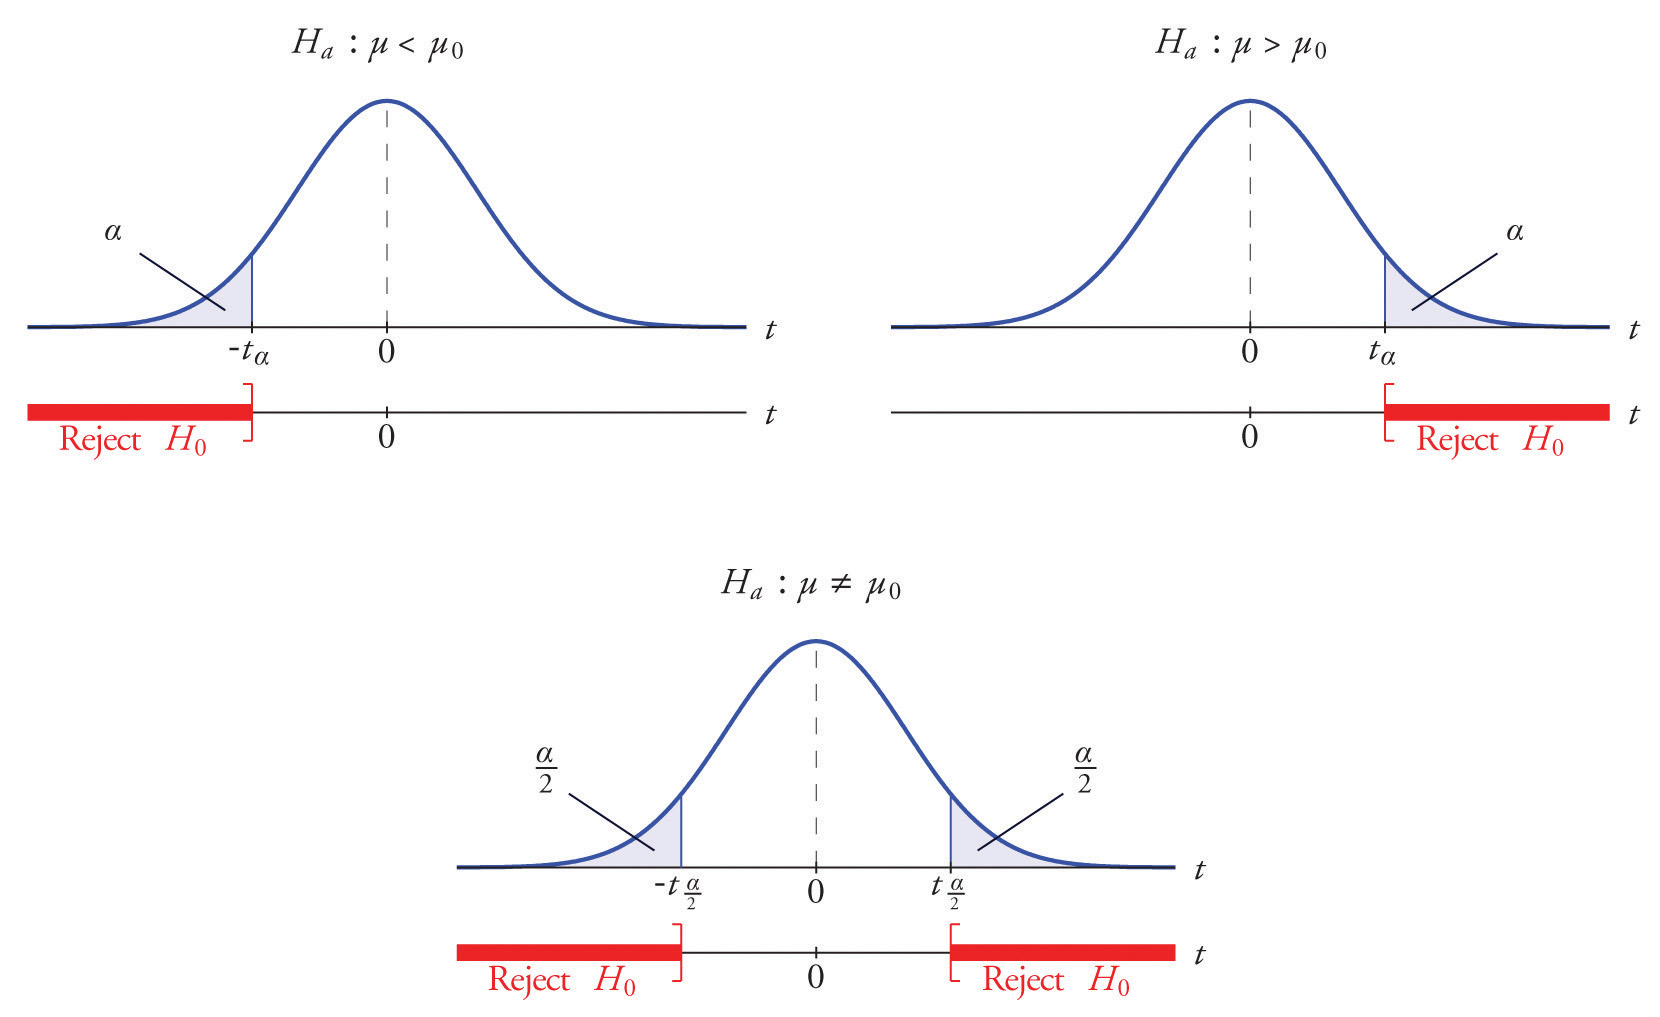
\includegraphics[height=2.2in]{HT1}
  \end{center}
\end{frame}

\begin{frame}
  \frametitle{Parametric versus nonparametric inference}
  \begin{itemize}
  \item What if the underlying distribution is not normal?
  \item Inference based on $t$-distribution \emph{may} be incorrect.
  \item It makes more sense to use a distribution-free statistical
    method, such as Wilcoxon rank-sum statistic, to perform the
    inference.
  \end{itemize}
\end{frame}

\begin{frame}
  \frametitle{Wilcoxon rank-sum statistic}
  \begin{itemize}
  \item The Wilcoxon rank-sum statistic is a nonparametric alternative
    to $t$-statistic:
    \begin{equation}
      \label{eq:wilcoxon}
      W = \sum^{n_1}_{j=1} r(x^{(A)}_{j})
    \end{equation}
  \item Where $r(x^{(A)}_{j})$ is the rank of $x^{(A)}_{j}$ in
    \emph{both groups}.
  \item The key point: only ranking information are needed, so
    \begin{enumerate}
    \item $p$-value computed from this statistic is valid even when
      the distribution of the expression levels are not normal.
      \cite{Gibbons1992NonparametricStatisticalInference}
    \item outliers have less effect to inference.
    \item Usually less powerful than its parametric counterpart.
    \end{enumerate}
  \end{itemize}
\end{frame}

\begin{frame}
  \frametitle{Other testing tools}
  \begin{itemize}
  \item There are many, many specialized tests design for many, many
    different type of problems.
  \item Examples:
    \begin{enumerate}
    \item Multiple group comparisons. One-way ANOVA
      $F$-test. Kruskal-Wallis test (nonparametric).
    \item Dependent data (as in pre/post analysis) group
      comparisons. Paired $t$-test; Friedman's test, etc.
    \item Binary data association (such as smoking and lung cancer).
      $\chi^{2}$-test and Fisher's exact test.
    \item Linear regression.  Goodness-of-fit $F$-test. $t$-test for
      linear association.
    \item Survival analysis. Log-rank test.
    \item Many, many more.
    \end{enumerate}
  \item If unsure, consult with a statistician for the most accurate
    and effective test for you data.
  \end{itemize}
\end{frame}

\section{Linear Regression Analysis}

\begin{frame}
  \frametitle{Why linear regression}
  This figure shows us an example in which we want to find out the
  \alert{linear relationship} between the covariate ($X$) and response
  ($Y$).
  \begin{center}
    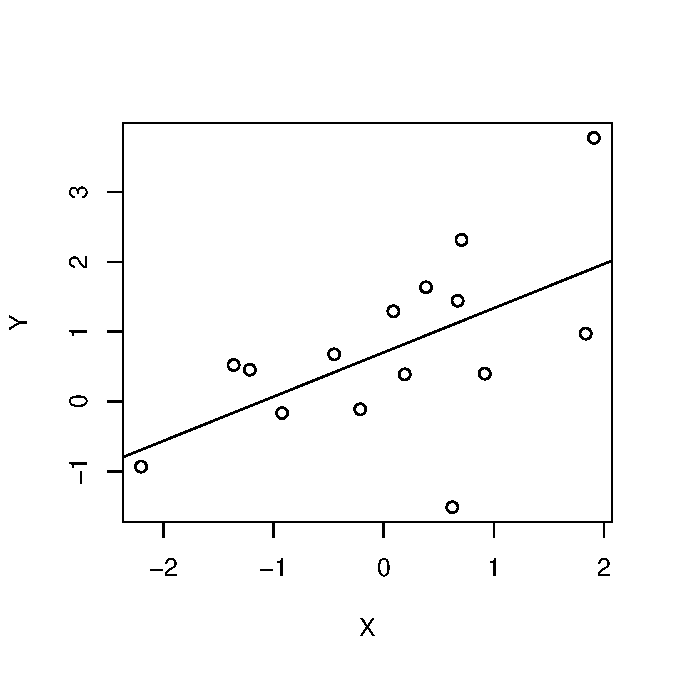
\includegraphics[height=2.2in]{lm-plot}
  \end{center}
\end{frame}

\begin{frame}
  \frametitle{Ordinary linear regression model}
  \begin{itemize}
  \item A simple linear model
    \begin{equation}
      \label{eq:simple-lin}
      Y = \beta_{0} + \beta_{1} X + \epsilon.
    \end{equation}
  \item A more general linear model is given as follows
    \begin{equation}
      \label{eq:lin}
      Y = \mathbf{X} \bm{\beta} + \epsilon.
    \end{equation}
  \item Here $X$ can be an $n\times p$-dimensional matrix. $n$ is the
    sample size, and $p$ is the number of covariates.  $Y$ is a vector
    of length $n$.  $\epsilon$ is a vector of errors.
  \item In many applications, we assume that $\epsilon_{i} \sim N(0,
    \sigma^{2})$ and they are independent.
  \end{itemize}
\end{frame}

\begin{frame}
  \frametitle{Inference of linear model}
  \begin{itemize}
  \item We can estimate $\beta_{j}$ by either maximum likelihood
    principle or minimizing the RSS.  These two approaches are
    equivalent under the normal $i.i.d.$ assumption.
  \item More than often, we also want to test the \alert{significance}
    of the linear association.
  \item The \emph{global} approach: Goodness-of-fit
    $F$-test. Essentially it is a signal-to-noise ratio.
  \item Once Goodness-of-fit $F$-test declares that there is an
    overall significant linear association between covariates and $Y$,
    we can use $t$-test to determine \alert{which} covariates
    contributed to this association.
  \end{itemize}
\end{frame}

\begin{frame}
  \frametitle{Model selection}
  \begin{itemize}
  \item If your goal is to build the best predictive model, using
    $p<0.05$ cut for individual covariates is not the best way.
  \item Marginally important variables may not be significant in
    multiple regression!
  \item Stepwise model selection based on AIC/BIC; $L^{1}$-penalized
    regression for high-dimensional regressions.
  \end{itemize}
\end{frame}

\begin{frame}
  \frametitle{Advanced Regression Models}
  \begin{itemize}
  \item General linear model, which allows non-independent
    $\epsilon$s.  Good for simple longitudinal analysis.
  \item Full-fledged linear mixed effect model.  You can model both
    fixed effect (like the covariates in an ordinal regression) and
    random effects (subject effect, time effect, batch effect, etc) in
    one model.
  \item Non-normal responses (such as binary or categorical
    responses).  Generalized linear model, possibly with random effect
    terms.  One of the most popular GLM is logistic regression.
  \item Nonparametric regression, \textit{a.k.a.} curve fitting.
  \item Other Specialized regression models, such as some time course
    regression models; spatial regression models, etc.
  \end{itemize}
\end{frame}



\begin{frame}
  \frametitle{Other Types of Statistical  Analyses}
  \begin{itemize}
  \item Data transformation.  $z$-transformation.  High-throughput data normalization.  Image registration.
  \item Dimension reduction.  Principal component analysis/factor analysis.
  \item Model-based cluster analysis.
  \item Discriminant analysis. Decision making.
  \item Network inference methods.
  \item Many, many other procedures!
  \end{itemize}
\end{frame}

\begin{frame}[allowframebreaks]{Bibliography}
  \bibliographystyle{amsplain}
  \bibliography{xing}
\end{frame}


%%% Local Variables:
%%% mode: latex
%%% TeX-master: "presentation"
%%% TeX-PDF-mode: t
%%% End:
